\documentclass[14pt,fleqn]{extarticle}
\RequirePackage{prepwell-eng}
\previewoff

\begin{document} 
\begin{snippet}
    
    \incorrect
    
    The region defined by 
    \[ \quad \left\lbrace (x,y): x \geq 0, x\leq y \leq \sqrt{4-x^2}\right\rbrace\]
    is as shown below 
    
    \begin{center}
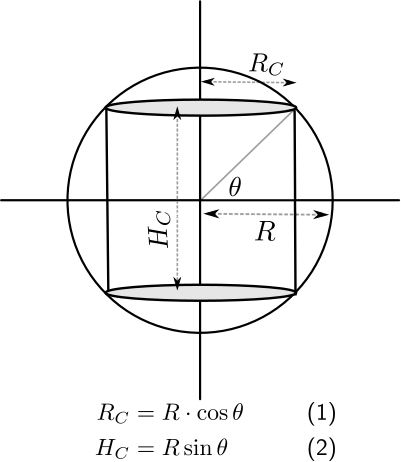
\includegraphics[scale=1.4]{wrong.svg}
\end{center}
    \reason
    
    We have been told which $(x,y)$ to consider in set-builder notation. And what we have been told is 
    
    \begin{center}
  \begin{tabular}{Nl}
   \toprule
        \text{Requirement} & Meaning \\
   \midrule 
   x\geq 0 & Points to the right of the origin \\
    \midrule 
    y\geq x & Above the line $x=y$ \\
    \midrule 
    y \leq \sqrt{4-x^2} & Inside the circle $x^2+y^2 = 4$ \\
    \bottomrule
  \end{tabular}
\end{center}

So, the required region is as shown below 
\begin{center}

\includegraphics[scale=1.4]{right.svg}
\end{center}
    
\end{snippet} 
\end{document} 